% Specify what kind of document this is
\documentclass[10pt, letterpaper]{article}


% Load extra packages to get access to special symbols and commands
\usepackage{fullpage}
\usepackage{color}
\usepackage{amsmath}
\usepackage{amssymb}
\usepackage{graphicx}
\usepackage{subfigure}

% Title information
\title{CS 224W Project Milestone}
\author{Nikhil Johri
  \and Zahan Malkani
  \and Ying Wang}
\date{}

% Begin
\begin{document}

\maketitle

\section{Introduction}
This project explores different models for building a recommendation system 
for Yelp.com. Yelp.com is a user review site where members comment on 
businesses within a metropolitan area. Some common types of businesses include 
restaurants, shopping, nightlife, and beauty spas. A reviewer assigns a 
star rating to a venue and writes a text review. Other members then have the 
opportunity to vote on the usefulness of the review (positive votes only).

Given a set of users, businesses and reviews, we aim to create a system that 
can predict, with reasonable accuracy, the rating a user would give 
to a business. We can evaluate our predictions over a set of held out data, 
and analyze the strengths and weaknesses of each models as a Yelp
recommendation system.


\section{Dataset}
The Yelp dataset consists of reviews of businesses around 30 universities. 
Each university region has about 250 businesses. Table \ref{stats} shows the 
main characteristics of our dataset. 

\begin{table}[htb]
\centering
\begin{tabular}{|c|c|}
\hline
Users &65,888 \tabularnewline \hline
Reviews &152,327 \tabularnewline \hline
Businesses &9600 \tabularnewline \hline
Reviews per user &Mean = 2.31, Median = 1, STD = 3.83 
\tabularnewline \hline
Reviews per business &Mean = 22.08, Median = 6, STD = 57.4 
\tabularnewline \hline
Average rating given &Mean = 3.64, Median = 4 \tabularnewline
in a review &Mode = 4, STD = 1.21 
\tabularnewline \hline

\end{tabular}
\caption{ Dataset statistics }
\label{stats}
\end{table}

From Table \ref{stats}, we see that our dataset is very sparse: over half of 
users have only reviewed one business. The spread of ratings is also not large: 
most reviews are assigned 4 stars (on an integer 1-5 scale), with standard 
deviation being a little over 1 star. To visualize review count distribution, 
we plot histograms for the review counts of both users and businesses in 
Figure \ref{review_count}. These two plots show that both distributions follow 
a power law, with a some irregularity at the beginning of the business' 
distribution. This happens because the number of businesses with only one 
rating happens to be low.

We randomly choose 10 percent of the reviews test set. Given a review 
from the test set, we look at the user and the business and make a predicted 
rating, which we compare to the actual rating. Each model's performance is 
evaluated using average root mean square error (RMSE) over the test set.


\begin{figure}[htb]
  \centering
  \subfigure[small][Users]
            {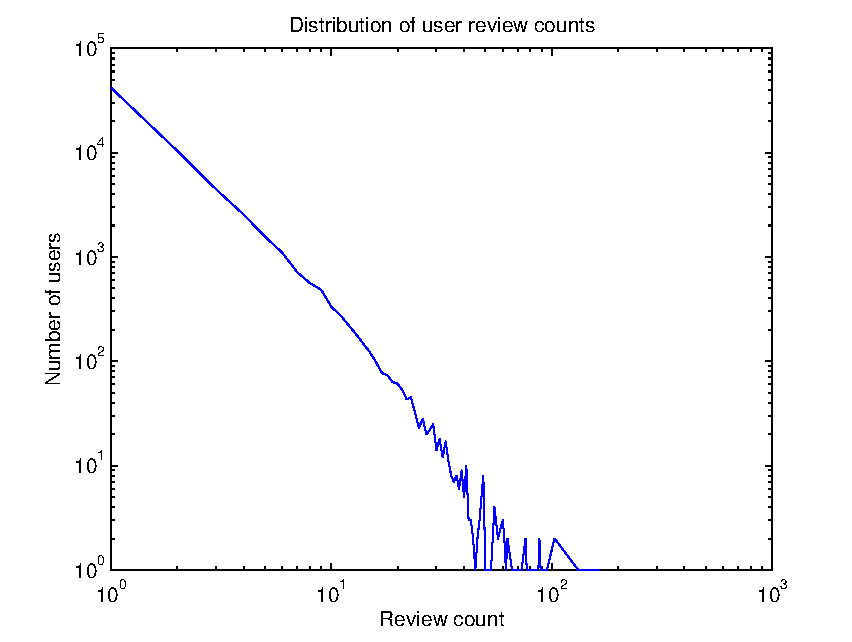
\includegraphics[width = 210pt]{images/u_hist.pdf}}
  \subfigure[small][Businesses]
            {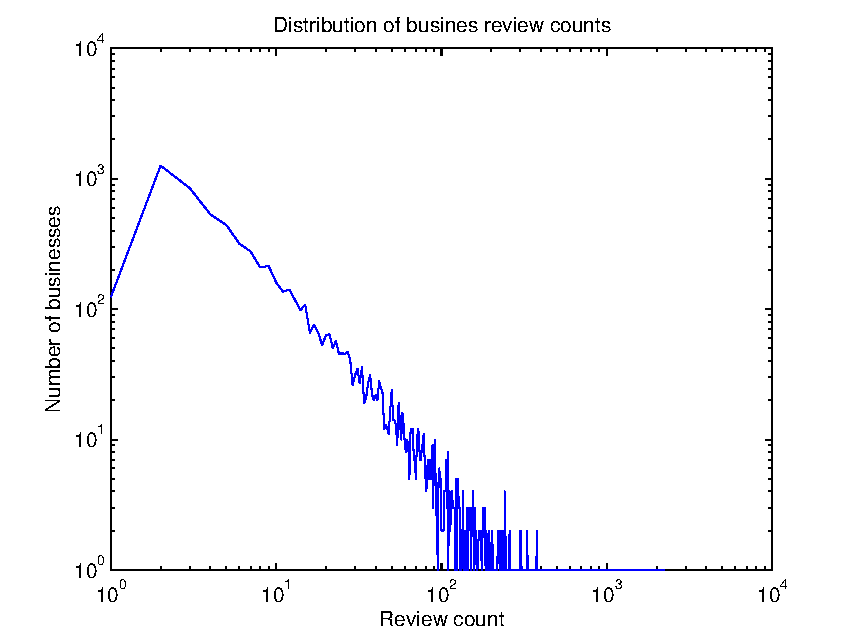
\includegraphics[width = 210pt]{images/b_hist.pdf}}

            \caption{Review count distributions}
            \label{review_count}

\end{figure}

\section{Neighborhood-based Collaborative Filtering}
In our first model, we use a neighborhood-based collaborative filtering method 
described as follows:
\begin{itemize}
\item Steps from project proposal go here. 
\end{itemize}

Mention that we use cosine similarity and because over half the users will have 
no basis for prediction, we predict ``4'' for them.

\begin{table}[htb]
\centering
\begin{tabular}{|c|c|}
\hline
{\bf Model} &{\bf RMSE} \tabularnewline \hline
Neighborhood-based CF &0.2032 \tabularnewline
Baseline (predict 4) &0.3454
\tabularnewline \hline

\end{tabular}
\caption{ Model Performance }
\label{ncf}
\end{table}


\end{document}
